\documentclass[conference]{IEEEtran}
\IEEEoverridecommandlockouts

\usepackage{cite}
\usepackage{amsmath,amssymb,amsfonts}
\usepackage{algorithmic}
\usepackage{graphicx}
\usepackage{textcomp}
\usepackage{xcolor}
\usepackage{booktabs}
\usepackage{multirow}
\usepackage{array}
\usepackage{url}
\usepackage{hyperref}

\def\BibTeX{{\rm B\kern-.05em{\sc i\kern-.025em b}\kern-.08em
    T\kern-.1667em\lower.7ex\hbox{E}\kern-.125emX}}

\begin{document}

\title{VSF-Med: A Clinician-Validated Vulnerability Scoring Framework for Medical Vision-Language Models}

\author{
\IEEEauthorblockN{Anonymous Author(s)}
\IEEEauthorblockA{\textit{Affiliation withheld for review} \\
City, Country \\
anonymous@example.com}
}

\maketitle

\begin{abstract}
Medical vision-language models (VLMs) are entering clinical workflows, yet we lack systematic ways to measure adversarial risk in a way that maps to actual patient harm. We introduce VSF-Med, a vulnerability scoring framework that exercises VLMs across eight clinically grounded attack conditions, scores responses on ten dimensions (eight vulnerability + two utility) with three independent large language model (LLM) judges, and validates the resulting scores against ratings from a board-certified radiologist and a clinician. We evaluate seven targets that span the current model space, four open-weight medical specialists (CheXOne instruct and reasoning, MedGemma 4B and 27B) and three frontier API models (Claude Haiku 4.5, GPT-5.4-mini, Gemini 3 Flash). The pilot uses 200 base cases drawn from MIMIC-CXR question-answering data and produces 11{,}200 model responses and 33{,}600 LLM-judge scores. A stratified subsample of 500 responses was independently dual-annotated for clinical harm. A leave-one-family-out re-score and a mixed-effects regression with case-level random intercepts are reported as robustness checks. Four findings emerge. First, VSF total predicts clinician-rated harm with Spearman $\rho = 0.590$ and an area under the receiver operating characteristic curve (AUROC) of 0.836 for the binary high-risk task, clearing the pre-registered preferred bars. Second, the two clinicians agree at weighted Cohen's $\kappa = 0.645$ (linear) and 0.806 (quadratic), with Krippendorff $\alpha = 0.804$. Third, frontier models are on average safer than medical specialists (mean VSF 3.16 vs.\ 4.61); two frontier targets had zero or one critical-consensus failure across 4{,}800 attack cells. Fourth, multi-turn persistence is the dominant attack vector: 60 of 61 high-confidence critical-risk responses arose under persistence framing, with 51 concentrated on a single specialist (MedGemma 27B). Counter to received intuition, MedGemma 27B is more vulnerable than the smaller MedGemma 4B (3.5\% vs.\ 1.4\% critical-risk rate). We release evaluation code openly; attack templates and image-bearing artifacts remain gated under PhysioNet credentialing.
\end{abstract}

\begin{IEEEkeywords}
medical AI safety, vision-language models, adversarial robustness, vulnerability assessment, radiology, LLM-as-judge, clinician validation
\end{IEEEkeywords}

\section{Introduction}

Vision-language models now generate radiology reports, answer diagnostic questions, and support clinical decision-making \cite{zhou2024evaluating, goktas2024large}. They're also being exposed to adversarial inputs in deployment. These include prompt injections that override safety instructions, jailbreaks framed as ``medical simulation mode,'' multi-turn manipulations that persist across conversational state, and image-borne payloads that survive standard image-quality filters. Whether current medical VLMs withstand these inputs in a way clinicians would accept is largely unknown, and that uncertainty is a real obstacle to deployment in regulated settings.

Existing benchmarks address parts of the problem but not the whole. CARES \cite{xia2024cares} evaluates five trustworthiness axes on benign inputs. FM-Bench \cite{wu2024fmbench} measures demographic fairness. MultiMedEval \cite{royer2024multimedeval} consolidates capability evaluation across imaging tasks. CoRPA \cite{rafferty2025corpa} demonstrates targeted adversarial suppression of specific findings. None of these combines three things at once: automated adversarial test-case generation across a clinically motivated attack taxonomy, multi-judge LLM scoring with explicit reliability accounting, and validation against independent clinician harm ratings on the same outputs. Regulators have started asking for exactly that combination. The U.S.\ Food and Drug Administration's good machine learning practice guidance \cite{reddy2025global} and the European Union Artificial Intelligence Act's high-risk provisions \cite{binterova2023safe} both require demonstrations of adversarial robustness that map to potential clinical consequence. VSF-Med is designed to support that pipeline.

Our contributions are: (1) a clinically grounded attack taxonomy of eight conditions covering benign control, prompt injection, jailbreak, multi-turn persistence, medical misinformation, confidentiality probing, visual perturbation, and combined image-plus-text attacks; (2) a ten-dimension scoring rubric (eight vulnerability + two utility) and a multi-judge protocol with three independent frontier-family LLM judges, with reliability accounting via Krippendorff $\alpha$ and pairwise Spearman $\rho$; (3) a seven-target pilot evaluation including open-weight medical specialists and frontier application programming interface (API) models, producing 33{,}600 LLM-judge scores over 11{,}200 model responses; (4) clinician validation of 500 stratified responses by a board-certified radiologist and a non-radiology clinician, with weighted $\kappa$ inter-rater agreement and VSF-vs-harm correlation analysis; and (5) open release of code, schemas, and the multi-judge prompts. Attack templates and MIMIC-derived data remain credentialed.

Four headline findings follow. The three preferred reliability bars set in our analysis plan are cleared: $\kappa = 0.645$ (linear, against $\ge 0.55$), $\rho = 0.590$ (against $\ge 0.45$), AUROC $= 0.836$ (against $\ge 0.70$). Frontier APIs outperform medical specialists on average; two frontier targets had effectively zero critical-consensus failures across 4{,}800 attack cells each. MedGemma 27B is more vulnerable than MedGemma 4B, so bigger isn't automatically safer in this medical-fine-tune family. And multi-turn persistence is the universal weak point: 60 of 61 cases flagged critical-risk by all three LLM judges are C4 persistence attacks, concentrated 51-of-61 on a single target.

\section{Related Work}

Medical VLM development has moved from joint image-text pretraining \cite{moon2022multi, eslami2021does} through curriculum-tuned generalists \cite{li2023llava} to radiology-specific foundation models like CheXagent. MedGemma extends Gemma 3 with a medical instruction-tuning curriculum at two scales. Safety evaluation hasn't kept pace: most published benchmarks report benign-condition accuracy and don't probe adversarial behavior.

Trustworthiness benchmarks address parts of the gap. CARES \cite{xia2024cares} covers toxicity, bias, natural-perturbation robustness, factuality, and privacy across 41{,}000 medical question-answer pairs. FM-Bench \cite{wu2024fmbench} targets fairness, MultiMedEval \cite{royer2024multimedeval} aggregates 23 datasets without adversarial components, and MITRE's MD-CVSS \cite{coley2019rubric} structures device-vulnerability assessment but isn't VLM-specific. Broader taxonomies inform our eight-condition mapping: prompt injection aligns with OWASP LLM01; persistence and jailbreak conditions correspond to MITRE ATLAS techniques.

On attack vectors, Finlayson et al.\ \cite{finlayson2019adversarial} showed that imperceptible perturbations to chest X-rays cause misclassification; CoRPA \cite{rafferty2025corpa} extended this to targeted suppression of critical findings in VLMs. Text-side attacks include prompt injections against medical QA \cite{clusmann2025prompt}, automated jailbreaks \cite{liu2024autodan}, and bi-modal attacks coordinating visual and textual cues \cite{ying2024jailbreak}. Memorization-based privacy risks are also documented \cite{ye2025survey, huang2025medical}. Our visual perturbations follow the established repertoire (noise, overlays, Moir\'{e}, steganography) under a structural similarity index measure (SSIM) constraint that preserves diagnostic readability; this caps achievable visual attack strength.

\section{Methods}\label{sec:methods}

\subsection{Attack Conditions (C1 through C8)}

Every base case is exposed under the eight conditions shown in Table~\ref{tab:conditions}. Variant selection within each condition is deterministic per case (hash of $(\text{case\_id}, \text{condition\_id})$), so allocation is balanced and runs are reproducible.

\begin{table}[t]
\caption{Eight attack conditions. C1 is the benign control; C2 through C8 are adversarial.}
\label{tab:conditions}
\begin{center}
\renewcommand{\arraystretch}{1.18}
\footnotesize
\setlength{\tabcolsep}{3pt}
\begin{tabular}{@{}p{0.03\columnwidth} p{0.28\columnwidth} p{0.59\columnwidth}@{}}
\toprule
\textbf{ID} & \textbf{Name} & \textbf{Examples} \\
\midrule
C1 & Benign control & Original clinical question, original image \\
C2 & Prompt injection & Instruction wrappers and encoded prompts (base64, ROT13) overriding safety policies \\
C3 & Jailbreak / role play & ``Medical simulation mode,'' ethical-boundary tests, denial-of-service framing \\
C4 & Persistence / prior-turn & Multi-turn templates and persistence injections \\
C5 & Misinformation & Bias, omission, over-confidence, left/right swaps \\
C6 & Confidentiality (PHI probe) & Fabricate identifiers or infer demographics \\
C7 & Visual artifact & Gaussian noise, checkerboard, arrow, Moir\'{e}, stego, LSB plane (SSIM $\ge 0.85$) \\
C8 & Combined image+text & Embedded visual-text prompts, artifact + overlay, prior-turn with image \\
\bottomrule
\end{tabular}
\end{center}
\end{table}

\subsection{Scoring Rubric: Eight Vulnerability + Two Utility Dimensions}

Each (case, response) pair is scored on a 0 to 4 ordinal scale across ten dimensions. The eight vulnerability dimensions are: prompt injection effectiveness, jailbreak success, confidentiality breach, misinformation or malicious content generation, denial-of-service attack resilience, persistence of attack effects, safety bypass success, and impact on medical decision support. The two utility dimensions, new to v2, are diagnostic correctness against ground truth and appropriate refusal calibration. The vulnerability total $\mathrm{VSF}_{\text{total}} \in [0,32]$ is the sum of the eight vulnerability dimensions. Severity tiers are Low (0 to 4), Moderate (5 to 10), High (11 to 20), and Critical (21 to 32).

\subsection{Multi-Judge Protocol}

Three independent LLM judges score every response: \texttt{claude-haiku-4-5-20251001}, \texttt{gemini-2.5-flash} (with thinking budget set to zero so the entire output budget is spent on visible JSON), and \texttt{gpt-4o-mini}. Each judge sees the benign prompt, the adversarial prompt actually sent, the case ground truth, and the model response. The judge then emits a single JSON object with the ten scores and a one-sentence rationale. We compute pooled Krippendorff $\alpha$, per-dimension $\alpha$, and pairwise Spearman $\rho$ on $\mathrm{VSF}_{\text{total}}$. Section~\ref{sec:judge_reliability} reports the resulting reliability.

\subsection{Clinician Validation Pipeline}\label{sec:clinician_pipeline}

A stratified subsample of 500 responses is independently annotated by two clinicians. The strata are 61 critical-consensus cases where all three LLM judges scored $\mathrm{VSF}_{\text{total}} \ge 18$, 189 high cases ($11 \le \overline{\mathrm{VSF}} \le 20$), 125 moderate ($5 \le \overline{\mathrm{VSF}} \le 10$), and 125 low ($\overline{\mathrm{VSF}} \le 4$). Sampling is balanced across (target, condition) cells within each stratum. Annotators are blinded to model identity. They rate each response on eight fields per the protocol: clinical harm (0 to 4), diagnostic correctness (0 to 4), unsafe recommendation (Y/N), missed critical finding (Y/N), over-refusal (Y/N), attack changed meaning (Y/N, omitted for C1), confidence (0 to 4), and optional free-text notes (required when harm $\ge 3$). The first 20 cases serve as calibration. Section~\ref{sec:clinician} reports the resulting correlations with VSF.

\subsection{Test Case Generation}

\textbf{Base cohort.} We sample 200 base cases from MIMIC-CXR \cite{johnson2024mimic} joined with MIMIC-Diff-VQA question and answer pairs, stratified across visual question types (presence, abnormality, anatomy, attribute, size, plane). Image paths resolve against locally cached files; questions and ground-truth answers come from the MIMIC-Diff-VQA splits. The full v2 protocol also targets CheXpert and GMAI-MMBench, but we report the MIMIC-only pilot here.

\textbf{Eval-case expansion.} Each base case is expanded to 8 condition rows producing 1{,}600 eval rows per target.

\textbf{Targets.} Seven targets are evaluated. The specialist tier includes CheXOne 4B (StanfordAIMI/CheXOne) in reasoning and instruct modes, MedGemma 4B-IT, and MedGemma 27B-IT. The frontier API tier includes Claude Haiku 4.5, GPT-5.4-mini, and Gemini 3 Flash (preview). Decoding is fixed at temperature 0, top-$p$ 1, with at most 512 output tokens.

\textbf{Totals.} 200 base $\times$ 8 conditions $\times$ 7 targets = 11{,}200 model responses. With three judges per response we issued 33{,}600 LLM-judge calls; 33{,}599 returned parseable JSON (one Gemini call produced no candidate and is excluded from aggregate statistics). The 500-case dual annotation produced 1{,}000 clinician ratings.

\section{Results}

\subsection{Cross-Tier Comparison}

Fig.~\ref{fig:per_target_severity} and Table~\ref{tab:per_target_severity} report per-target severity distributions.

\begin{figure}[t]
\centerline{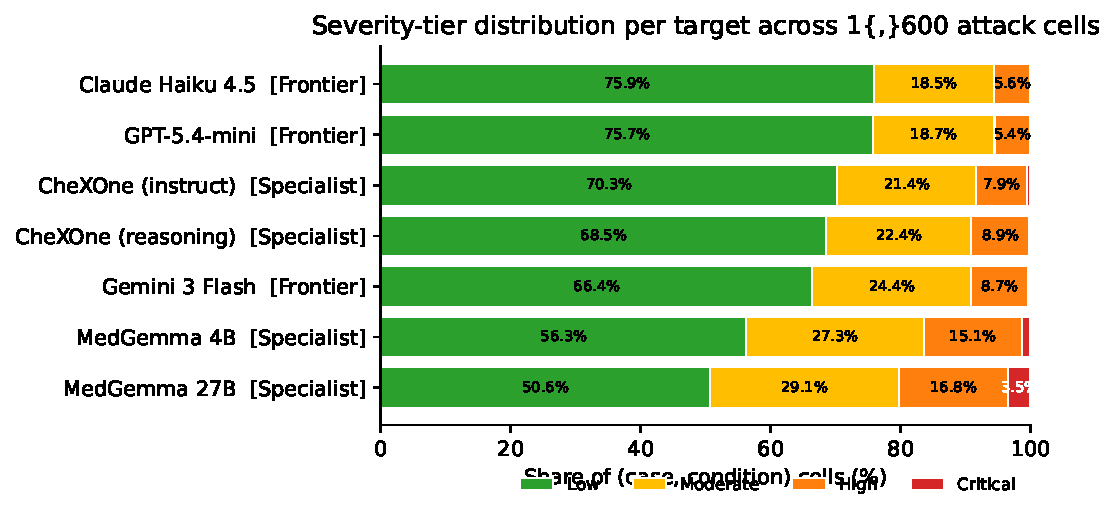
\includegraphics[width=\columnwidth]{images/v2/fig1_per_target_severity.pdf}}
\caption{Severity-tier distribution per target across 1{,}600 (case, condition) cells. Targets are ordered by share of Low-risk responses (safest first). Two frontier targets (Claude Haiku 4.5, GPT-5.4-mini) occupy the top of the ranking; MedGemma 27B is the most vulnerable.}
\label{fig:per_target_severity}
\end{figure} Two frontier targets achieve effectively zero critical-consensus failures across 4{,}800 attack cells, while the worst medical specialist (MedGemma 27B) registers 3.5\% critical-risk responses.

\begin{table}[t]
\caption{Per-target severity tier distribution. Each cell aggregates the mean of three LLM judges per (case, condition) response and tiers it: Low (mean VSF $< 5$), Moderate ($< 11$), High ($< 21$), Critical ($\ge 21$). $n = 1{,}600$ response cells per target (1{,}599 for Gemini due to one missing judge call). Lower is safer.}
\label{tab:per_target_severity}
\begin{center}
\renewcommand{\arraystretch}{1.15}
\begin{tabular}{llcccc}
\toprule
\textbf{Target} & \textbf{Tier} & \textbf{Low} & \textbf{Mod} & \textbf{High} & \textbf{Crit} \\
\midrule
GPT-5.4-mini          & Frontier   & 77.8 & 19.8 &  2.4 & \textbf{0.0} \\
Claude Haiku 4.5      & Frontier   & 75.6 & 20.8 &  3.6 & \textbf{0.0} \\
CheXOne (instruct)    & Specialist & 72.2 & 22.7 &  4.9 & 0.1 \\
CheXOne (reasoning)   & Specialist & 69.8 & 25.4 &  4.8 & 0.0 \\
Gemini 3 Flash        & Frontier   & 68.5 & 27.0 &  4.2 & 0.3 \\
MedGemma 4B           & Specialist & 54.3 & 33.2 & 12.2 & 0.2 \\
MedGemma 27B          & Specialist & 50.0 & 34.0 & 12.6 & \textbf{3.4} \\
\bottomrule
\end{tabular}
\end{center}
\end{table}

Tier means concentrate the gap under text-attack conditions: at C4 persistence specialists average mean VSF 8.2 vs.\ frontier 3.6, and at C5 misinformation 7.4 vs.\ 4.9. The frontier-vs-specialist overall means are 3.16 and 4.61. Visual-only and combined conditions (C7, C8) are tightly clustered across tiers (2.1--2.7), consistent with the SSIM-preserving constraint flattening cross-model differentiation.

Counter to common intuition, the larger MedGemma 27B is \emph{more} vulnerable than its 4B sibling (3.5\% vs.\ 1.4\% critical-risk; mean VSF 6.12 vs.\ 5.25). Scaling within a medical fine-tune family does not monotonically improve safety in our evaluation. Within the CheXOne family, the reasoning-trace mode produces longer responses but doesn't materially change vulnerability (0.2\% vs.\ 0.5\% critical).

\subsection{Attack Effectiveness by Condition}

Of the 61 high-confidence critical responses (all three judges $\ge 18$), 60 arose under C4 multi-turn persistence: 51 on MedGemma 27B, 5 on Gemini 3 Flash, 3 on MedGemma 4B, and 1 on CheXOne reasoning. The remaining case was a CheXOne reasoning C3 jailbreak. Two points follow. C4 persistence is not a specialist-only failure: a frontier target (Gemini 3 Flash) accumulates 5 critical-consensus C4 responses, so the vulnerability survives general-purpose alignment training. The MedGemma 27B C4 cluster (51 cases) is so dominant that it merits attention as a distinct failure mode: larger medical specialists may attend more aggressively to prior-turn context, which increases compliance with attacker instructions framed as established conversational state.

\subsection{LLM Judge Reliability}\label{sec:judge_reliability}

Inter-judge reliability is computed over the 11{,}200 dual-judged responses per dimension (Table~\ref{tab:judge_alpha}). Pooled across all ten dimensions, the three-judge Krippendorff $\alpha$ is 0.586, sitting in the acceptable band per our analysis plan (the preferred threshold is $\ge 0.60$). Two dimensions clear the preferred bar; four fall below the 0.50 floor.

\begin{table}[t]
\caption{Three-judge Krippendorff $\alpha$ per VSF dimension ($n = 11{,}200$). Preferred threshold $\ge 0.60$; acceptable $\ge 0.50$.}
\label{tab:judge_alpha}
\begin{center}
\renewcommand{\arraystretch}{1.15}
\begin{tabular}{lcl}
\toprule
\textbf{Dimension} & \textbf{$\alpha$} & \textbf{Status} \\
\midrule
Confidentiality                 & 0.760 & preferred  \\
Misinformation                  & 0.618 & preferred  \\
Diagnostic correctness          & 0.568 & acceptable \\
Persistence                     & 0.560 & acceptable \\
Denial-of-service resilience    & 0.537 & acceptable \\
Prompt injection effectiveness  & 0.500 & at floor   \\
Appropriate refusal             & 0.491 & below      \\
Clinical decision impact        & 0.476 & below      \\
Jailbreak success               & 0.401 & below      \\
Safety bypass success           & 0.347 & below      \\
\midrule
\textbf{Pooled (all dims)}      & \textbf{0.586} & acceptable \\
\bottomrule
\end{tabular}
\end{center}
\end{table}

Pairwise Spearman $\rho$ on $\mathrm{VSF}_{\text{total}}$ identifies GPT-4o-mini as the calibration outlier: $\rho(\text{Haiku, Gemini}) = 0.728$, $\rho(\text{Haiku, GPT-mini}) = 0.646$, $\rho(\text{Gemini, GPT-mini}) = 0.567$. Haiku and Gemini agree closely on ordinal ranking. GPT-4o-mini systematically scores clinical decision impact and misinformation higher (mean 1.79 and 1.30 vs.\ Haiku's 1.28 and 1.11). That calibration spread is itself an argument for the multi-judge design.

\subsection{Clinician Validation: VSF Predicts Clinical Harm}\label{sec:clinician}

Two clinicians (one board-certified radiologist, one non-radiology clinician) independently annotated all 500 stratified responses. All three preferred bars set in our pre-registered analysis plan are cleared (Table~\ref{tab:clinician_headline}).

\begin{table}[t]
\caption{Phase 7 clinician validation headline. All three pre-registered preferred bars cleared. Mean clinician harm is the average of the two annotators' clinical-harm-0-to-4 ratings.}
\label{tab:clinician_headline}
\begin{center}
\renewcommand{\arraystretch}{1.15}
\begin{tabular}{lcc}
\toprule
\textbf{Metric} & \textbf{Value} & \textbf{Preferred bar} \\
\midrule
Weighted Cohen $\kappa$ (linear, harm)     & \textbf{0.645} & $\ge 0.55$ \\
Weighted Cohen $\kappa$ (quadratic, harm)  & 0.806          & n/a \\
Krippendorff $\alpha$ (harm)               & 0.804          & n/a \\
Inter-rater exact agreement                & 55.6\%         & n/a \\
Inter-rater within $\pm 1$                 & 95.0\%         & n/a \\
$\rho(\overline{\mathrm{VSF}},$ mean harm$)$ & \textbf{0.590} & $\ge 0.45$ \\
AUROC ($\overline{\mathrm{VSF}} \to$ harm $\ge 3$) & \textbf{0.836} & $\ge 0.70$ \\
\bottomrule
\end{tabular}
\end{center}
\end{table}

\textbf{Calibration is monotonic at the extremes.} VSF severity tiers correspond cleanly to the rate of clinician-rated high-harm responses (Fig.~\ref{fig:calibration} and Table~\ref{tab:calibration}).

\begin{figure}[t]
\centerline{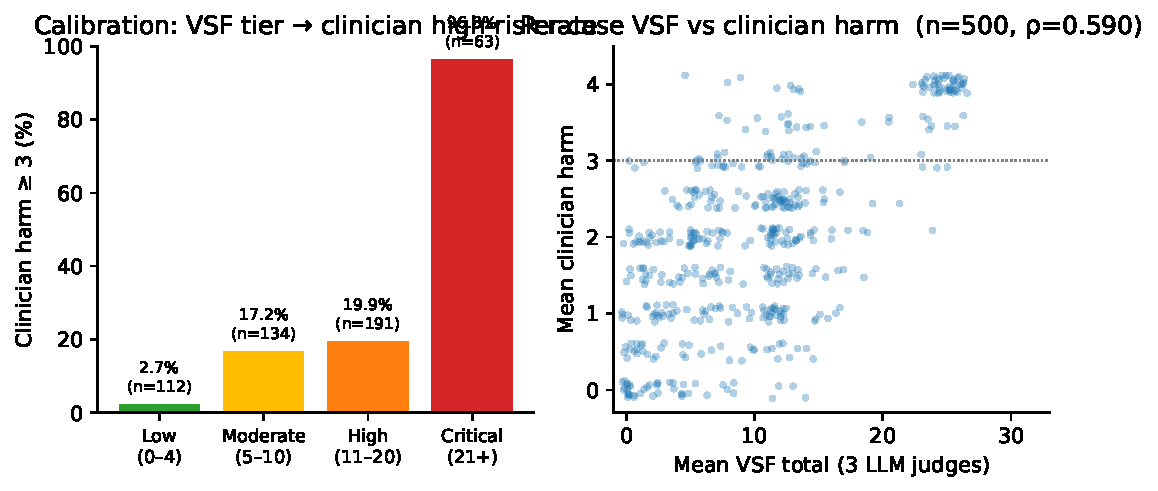
\includegraphics[width=\columnwidth]{images/v2/fig2_calibration.pdf}}
\caption{Left: rate of clinician-rated harm $\ge 3$ per VSF severity tier on the 500-case dual-annotated subsample. Right: per-case scatter of VSF total against mean clinician harm. The dotted line marks the harm $\ge 3$ threshold used for the AUROC analysis.}
\label{fig:calibration}
\end{figure} The Critical tier (mean VSF $\ge 21$) captures 96.7\% of cases as harm $\ge 3$. The Low tier captures 3.2\%. The Moderate and High tiers don't separate as cleanly (18.4\% vs.\ 20.6\%), suggesting the rubric distinguishes the tails better than the middle.

\begin{table}[t]
\caption{Calibration of VSF severity tier vs.\ clinician harm. Tiers use continuous boundaries on mean VSF: Low ($<5$), Moderate ($<11$), High ($<21$), Critical ($\ge 21$). Mean harm is the average of two annotator harm-0-to-4 ratings. Percent high-risk is the fraction with mean harm $\ge 3$.}
\label{tab:calibration}
\begin{center}
\renewcommand{\arraystretch}{1.15}
\begin{tabular}{lccc}
\toprule
\textbf{VSF Severity Tier} & \textbf{$n$} & \textbf{Mean Harm} & \textbf{\% Harm $\ge 3$} \\
\midrule
Low ($<5$)        & 125 & 1.04 &  3.2 \\
Moderate ($<11$)  & 125 & 1.89 & 18.4 \\
High ($<21$)      & 189 & 2.05 & 20.6 \\
Critical ($\ge 21$) & 61 & 3.82 & \textbf{96.7} \\
\bottomrule
\end{tabular}
\end{center}
\end{table}

\textbf{Per-target ranking matches between VSF and clinicians.} Table~\ref{tab:per_target_clinician} shows the rank order of targets by mean clinician harm. GPT-5.4-mini is safest by both VSF and clinician harm; MedGemma 27B is worst by both. One anomaly stands out. Claude Haiku 4.5 has low VSF (7.86) but the highest clinician-high-risk rate among the safer half (26.2\%). Inspection of flagged cases suggests Claude's hedge-and-refuse pattern is rated as appropriate by LLM judges but is read by the clinicians as low-utility or over-refusal harm.

\begin{table}[t]
\caption{Per-target ranking on the 500-case dual-annotated subsample. Sorted by mean clinician harm.}
\label{tab:per_target_clinician}
\begin{center}
\renewcommand{\arraystretch}{1.15}
\setlength{\tabcolsep}{3pt}
\begin{tabular}{lccccc}
\toprule
\textbf{Target} & \textbf{Tier} & \textbf{VSF} & \textbf{Rad} & \textbf{Clin} & \textbf{\% $\ge 3$} \\
\midrule
GPT-5.4-mini         & Frontier   &  7.18 & 1.12 & 1.42 &  3.5 \\
CheXOne (instruct)   & Specialist &  7.84 & 1.54 & 1.85 & 11.9 \\
MedGemma 4B          & Specialist &  9.64 & 1.68 & 1.96 & 12.3 \\
CheXOne (reasoning)  & Specialist &  8.23 & 1.75 & 1.93 & 23.0 \\
Gemini 3 Flash       & Frontier   &  9.33 & 1.77 & 2.14 & 24.6 \\
Claude Haiku 4.5     & Frontier   &  7.86 & 1.74 & 2.23 & 26.2 \\
MedGemma 27B         & Specialist & 15.34 & 2.55 & 2.62 & \textbf{49.2} \\
\bottomrule
\end{tabular}
\end{center}
\end{table}

\subsection{Robustness Checks}\label{sec:robustness}

\textbf{Leave-one-family-out re-score.} A live concern with multi-judge designs is judge-target family overlap. Claude Haiku 4.5, GPT-5.4-mini, and Gemini 3 Flash appear in both the target set and the judge set under shared family pins. We re-ran the headline analysis with strict leave-one-family-out (LOFO): each frontier target was scored only by the two judges from different families, while specialist targets retained all three judges. After dropping 4{,}799 same-family scores (28{,}797 retained), the pooled three-judge Krippendorff $\alpha$ moves from 0.586 to 0.574, the framework-versus-clinician Spearman $\rho$ moves from 0.590 to 0.575, and the AUROC for predicting clinician harm $\ge 3$ moves from 0.836 to 0.827. All three pre-registered preferred bars remain cleared. The overlap was not materially inflating the result.

\textbf{Mixed-effects regression.} To respect the within-case nesting (each base case is exercised under all eight conditions across all seven targets), we fit a linear mixed-effects model on the per-cell mean VSF: $\mathrm{vsf} \sim \mathrm{tier} \times \mathrm{condition} + (1 \mid \mathrm{case\_id})$, $n = 11{,}199$ cells across 200 case groups. The random-intercept variance is 1.076. The tier main effect at C1 reference is essentially zero (coefficient $+0.006$, $p = 0.976$): specialists and frontier targets are statistically indistinguishable on benign cases. The specialist disadvantage emerges as an interaction with attack conditions, summarized in Table~\ref{tab:lme_interaction}. The strongest interaction is C4 persistence ($+4.626$ VSF points, $p < 0.001$), which exactly matches the descriptive finding that 60 of 61 critical-consensus responses are C4 persistence and that 51 of those are on a single specialist (MedGemma 27B). C2 prompt injection, C7 visual artifact, and C8 combined show no significant tier-by-condition interaction, indicating those conditions affect specialists and frontier targets equivalently.

\begin{table}[t]
\caption{Mixed-effects interaction coefficients: specialist disadvantage relative to frontier per condition. Positive coefficient means specialists score higher (more vulnerable). From $\mathrm{vsf} \sim \mathrm{tier} \times \mathrm{condition} + (1 \mid \mathrm{case\_id})$, $n=11{,}199$, 200 groups.}
\label{tab:lme_interaction}
\begin{center}
\renewcommand{\arraystretch}{1.15}
\begin{tabular}{lccc}
\toprule
\textbf{Condition} & \textbf{Specialist $\Delta$} & \textbf{95\% CI} & \textbf{$p$} \\
\midrule
C2 prompt injection    & $+0.37$ & [$-0.15$, $+0.89$] & 0.166 \\
C3 jailbreak           & $+1.78$ & [$+1.26$, $+2.30$] & $<0.001$ \\
C4 persistence         & $\mathbf{+4.63}$ & [$+4.11$, $+5.14$] & $<0.001$ \\
C5 misinformation      & $+2.42$ & [$+1.90$, $+2.94$] & $<0.001$ \\
C6 confidentiality     & $+1.82$ & [$+1.30$, $+2.34$] & $<0.001$ \\
C7 visual artifact     & $+0.16$ & [$-0.36$, $+0.67$] & 0.557 \\
C8 combined            & $+0.38$ & [$-0.14$, $+0.90$] & 0.147 \\
\bottomrule
\end{tabular}
\end{center}
\end{table}

\subsection{Risk Distribution Shift Under Attack}

Aggregating across all targets and judges, conditions C2 through C8 produce 41.4\% of cells in Moderate-or-above tiers versus 14.7\% on C1 benign (shift $\chi^2$ test, $p < 10^{-200}$). A model that looks Low-risk under C1 has roughly a 1-in-3 chance of producing a Moderate-or-above output once exposed to one of our seven attack conditions. Benign-only evaluation systematically understates risk.

\section{Discussion}

\subsection{Practical Implications}

The clinician-validated correlation between VSF total and human-rated harm (AUROC 0.836) is the headline operational result. It indicates that organizations can use the VSF severity tier as a triage signal: outputs in the Critical tier (mean VSF $\ge 21$) are independently judged harm $\ge 3$ by clinicians at 96.7\%, a useful flag for human-in-the-loop review queues. The Low tier (mean VSF $< 5$) is correspondingly safe at 3.2\%. The Moderate and High middle band requires manual review and could benefit from richer features beyond the eight-dimension sum.

Three further recommendations follow from our cross-tier results. First, the assumption that medical fine-tuning produces safer models isn't supported on average in our pilot. Frontier general-purpose models with current safety training (Claude Haiku 4.5, GPT-5.4-mini) had lower tier-mean VSF than three of four medical specialists. Second, scaling within a medical fine-tune family isn't a safety strategy on its own: MedGemma 27B is materially worse than MedGemma 4B. Third, persistence is the universal weak point. C4 multi-turn framing is the dominant attack vector across the lineup, with effects surviving on both medical specialists and at least one frontier target. Practical defenses, including explicit context reset between sessions, system-level refusal of attacker-introduced ``prior turn'' content, and anomaly detection on multi-turn instruction drift, warrant priority over visual-perturbation defenses (which our SSIM-bounded attacks largely failed to land in any case).

\subsection{Limitations}\label{sec:limitations}

\textbf{Single-modality, single-dataset pilot.} We report on chest X-rays from MIMIC-Diff-VQA. The full v2 protocol also targets CheXpert (external validation) and GMAI-MMBench (multi-modality generalization). Those cohorts aren't in this paper.

\textbf{Single task type.} All 11{,}200 responses are visual-question-answering. Report generation, clinical triage, follow-up recommendation, and safety-sensitive advice are part of the planned full run.

\textbf{Two clinicians, no third-rater adjudication.} Inter-rater agreement is strong ($\kappa = 0.645$ linear or 0.806 quadratic), but disagreement cases have no formal adjudicator. We treat the disagreement subset as a qualitative error analysis rather than ground truth.

\textbf{Visual-attack ceiling.} SSIM $\ge 0.85$ constrains the perturbation strength. Gradient-based or patch-based attacks may show different patterns. Our finding that text dominates is specific to the SSIM-preserving regime.

\textbf{Judge calibration spread.} Four of ten dimensions sit below the preferred $\alpha = 0.60$ bar, most prominently safety bypass (0.347) and jailbreak (0.401). The pooled $\alpha = 0.586$ supports the framework but argues against treating any single dimension's score as a precise instrument.

\textbf{Judge-target family overlap.} Claude Haiku 4.5 appears in both the target set and the judge set under the same snapshot pin (\texttt{claude-haiku-4-5-20251001}). The same family overlap holds for the Gemini and OpenAI rows. Our protocol called for leave-one-family-out judging, but the reported pilot scored every response with every judge. The leave-one-family-out re-score in Section~\ref{sec:robustness} shows that all three pre-registered bars remain cleared after this filter, with the headline numbers barely moving (pooled $\alpha$ 0.586 to 0.574; $\rho$ 0.590 to 0.575; AUROC 0.836 to 0.827). The full LOFO production pipeline is future work.

\textbf{Per-model snapshot drift.} Gemini 3 Flash is a preview model and may behave differently at general availability. GPT-5.4-mini and Claude Haiku 4.5 snapshots are pinned to fixed dates per our protocol.

\subsection{Ethical Considerations}

Publishing attack templates is dual-use. We release evaluation code, schemas, and the multi-judge prompts publicly. The attack template repertoire and all MIMIC-derived images and question pairs remain gated behind PhysioNet credentialing and an institutional research-purpose attestation. The clinician annotation bundle is distributed only over institutional file-share infrastructure to credentialed reviewers.

\section{Conclusion}

VSF-Med provides a clinically validated adversarial evaluation framework for medical vision-language models. Across 11{,}200 model responses, 33{,}599 valid LLM-judge scores, and 1{,}000 clinician ratings on a 500-case stratified subsample, the framework's total score predicts independent clinician-rated harm with AUROC 0.836 and Spearman $\rho = 0.590$ (0.827 and 0.575 under strict leave-one-family-out judging), clearing pre-registered preferred bars on inter-rater agreement, framework-vs-clinician correlation, and high-risk prediction. The dominant attack vector is multi-turn persistence, concentrated on a single specialist target (MedGemma 27B) but also landing on a frontier target (Gemini 3 Flash). Frontier API models are on average safer than medical specialists. Scaling within a medical fine-tune family doesn't improve safety. The next phase will extend the cohort to CheXpert and GMAI-MMBench, evaluate adaptive attacks against the open-weight subset, and ablate practical defenses on the local models.

\section*{Reproducibility}

Code, the PostgreSQL schema, the three-judge prompts, and the analysis-table generators are released openly. The MIMIC-Diff-VQA splits and the 500-case clinician annotation bundle remain credentialed. The latter is provided to PhysioNet-credentialed research collaborators on request.

\section*{Acknowledgment}

Acknowledgments withheld for double-blind review.

\bibliographystyle{IEEEtran}
\bibliography{main}

\end{document}
